\documentclass[12pt, letterpaper]{article}
\usepackage{amsmath}
\usepackage{amssymb}
\usepackage{latexsym}
\usepackage[usenames,dvipsnames]{xcolor}
\usepackage{graphicx}
\usepackage[headheight=15pt, margin=2.5cm]{geometry}
\usepackage{setspace}
\usepackage{longtable}
\usepackage{pdflscape}
\usepackage{ctable}
\usepackage{booktabs}
\usepackage{caption}
\usepackage{subcaption}
\usepackage[binary-units=true]{siunitx}
\usepackage{enumitem}
\usepackage{multirow}
\usepackage{float}
\usepackage{hhline}
\usepackage{tabulary}
\usepackage[nottoc, notlof, notlot]{tocbibind}
\usepackage[framed]{mcode}
%\usepackage{indentfirst}
\usepackage{standalone}
\usepackage{fancyhdr}
\usepackage{array}
\newcolumntype{P}[1]{>{\raggedright\arraybackslash}p{#1}}
\lstset{breaklines}
\usepackage[hyphens]{url}
\usepackage{cleveref}
\setlength{\parindent}{0em}
%\renewcommand{\baselinestretch}{1.3}

\pagestyle{fancy}
\fancyhf{}
\lhead{SRK}
\rhead{Mechanical Design}

\begin{document}
%%%%%%%%%%%%%%%%%%%%%%%%%%%%%%%%%%%%%%%%%
% University Assignment Title Page 
% LaTeX Template
% Version 1.0 (27/12/12)
%
% This template has been downloaded from:
% http://www.LaTeXTemplates.com
%
% Original author:
% WikiBooks (http://en.wikibooks.org/wiki/LaTeX/Title_Creation)
%
% License:
% CC BY-NC-SA 3.0 (http://creativecommons.org/licenses/by-nc-sa/3.0/)
% 
% Instructions for using this template:
% This title page is capable of being compiled as is. This is not useful for 
% including it in another document. To do this, you have two options: 
%
% 1) Copy/paste everything between \begin{document} and \end{document} 
% starting at \begin{titlepage} and paste this into another LaTeX file where you 
% want your title page.
% OR
% 2) Remove everything outside the \begin{titlepage} and \end{titlepage} and 
% move this file to the same directory as the LaTeX file you wish to add it to. 
% Then add \input{./title_page_1.tex} to your LaTeX file where you want your
% title page.
%
%%%%%%%%%%%%%%%%%%%%%%%%%%%%%%%%%%%%%%%%%

%----------------------------------------------------------------------------------------
%	PACKAGES AND OTHER DOCUMENT CONFIGURATIONS
%----------------------------------------------------------------------------------------

\documentclass[12pt]{article}
\usepackage[margin=2.5cm]{geometry}

\begin{document}

\newcommand{\HRule}{\rule{\linewidth}{0.5mm}} % Defines a new command for the horizontal lines, change thickness here
\begin{titlepage}


\center % Center everything on the page
 
%----------------------------------------------------------------------------------------
%	HEADING SECTIONS
%----------------------------------------------------------------------------------------

\textsc{\LARGE University of Toronto}\\[1.2cm] % Name of your university/college
\textsc{\Large AER407 - Space Systems Design}\\[0.5cm] % Major heading such as course name
\textsc{\large Space Robo Korporation}\\[0.5cm] % Minor heading such as course title

%----------------------------------------------------------------------------------------
%	TITLE SECTION
%----------------------------------------------------------------------------------------

\HRule \\[0.4cm]
{ \huge \bfseries Mechanical Design for Canada's Next Generation Robotics}\\[0.5cm] % Title of your document
\HRule \\[1.2cm]

%----------------------------------------------------------------------------------------
%	LOGO SECTION
%----------------------------------------------------------------------------------------


\includegraphics[width=0.4\textwidth]{logo}\\[1cm] 

%----------------------------------------------------------------------------------------
%	AUTHOR SECTION
%----------------------------------------------------------------------------------------


\begin{centering} \large
\begin{tabular}{ll}
Mechanical	&	Jai Bansal (999856179)	\\
Electrical	& 	Hao Xing (999261345)	\\
Controls	&	Yun-Jae Kim (999870947)	\\
Operations	&	Guanchu Liu (999183011)	\\
Systems		&	Lian Liu (998700892)	\\[1cm]
\end{tabular}
\end{centering}


% If you don't want a supervisor, uncomment the two lines below and remove the section above
%\Large \emph{Author:}\\
%John \textsc{Smith}\\[3cm] % Your name

%----------------------------------------------------------------------------------------
%	DATE SECTION
%----------------------------------------------------------------------------------------

{\large \today}\\[3cm] % Date, change the \today to a set date if you want to be precise
 
%----------------------------------------------------------------------------------------

\vfill % Fill the rest of the page with whitespace

\end{titlepage}
\end{document}		%Cover page
\cfoot{\normalsize\thepage}
\pagenumbering{roman}% Roman-numbered pages (start from i)
\onehalfspacing
\newpage
\begin{document}

\section*{List of Symbols}

\begin{tabular}{ll}
\textbf{ATCS}	&	Active Thermal Control System	\\
\textbf{DOF}	&	Degrees of Freedom	\\
\textbf{EML2}	&	Earth-Moon Lagrange Point 2	\\
\textbf{ERA}	&	European Robotic Arm	\\
\textbf{EVA}	&	Extravehicular Activity	\\
\textbf{ISS}	&	International Space Station	\\
\textbf{MDA}	&	MacDonald, Dettwiler and Associates Ltd.	\\
\textbf{PAN}	&	Polyacrylonitrile	\\
\textbf{PTCS}	&	Passive Thermal Control System	\\
\textbf{RFP}	&	Request for Proposal	\\
\textbf{TBC}	&	To be confirmed	\\
\textbf{TBD}	&	To be determined	\\

\end{tabular}

\section*{List of Nomenclature}

\begin{tabular}{ll}
\textit{kg}	&	kilogram\\
\textit{m}	&	meter	\\
\textit{s}	&	second	\\
\textit{W}	&	Watt	\\
\textit{N}	&	Newton	\\
\textit{GB}	&	Gigabyte\\
\textit{lb}	&	pound	\\
\textit{\si{\celsius}}	&	degrees Celsius

\end{tabular}
\vspace*{\fill}

\newpage

\section*{Requirement Naming Convention}
\begin{tabular}{ll}
\textbf{System Requirement}:	&	S-F/P/C/E-XX	\\
\textbf{Subsystem Requirement}	&	LM-F/P/C/E-XX	\\
\end{tabular}\\
\vspace{10pt}

\begin{tabular}{ll}
\textbf{F}	&	Functional Requirement	\\
\textbf{P}	&	Performance Requirement	\\
\textbf{C}	&	Constraint Requirement	\\
\textbf{E}	&	Environmental Requirement	\\
\\
\textbf{LM}	&	Locomotion		\\
\textbf{DH}	&	Data Handling	\\
\textbf{TC}	&	Thermal Control	\\
\textbf{PS}	&	Power System	\\
\textbf{EE}	&	End Effector	\\
\textbf{SR}	&	Sensors			\\
\textbf{FM}	&	Frame			\\
\\
\textbf{XX}	&	Numbering for system/subsystem requirements\\
\end{tabular}

\vspace*{\fill}

\end{document}
\newpage
\begin{document}
\topskip0pt
\vspace*{\fill}
\begin{center}
\large
\textbf{Executive Summary}
\end{center}

\normalsize
The following document outlines the mechanical aspects of the robotic system and subsystems involved in the development and maintenance of a future lunar Outpost. Firstly, an overview of the mechanical aspects of each system is briefly tabulated and described. Then, the subsystem mechanical requirements are clearly defined, and sub-categorized appropriately into functional, or performance requirements. Next, the major mechanical trade-offs are discussed, including the architecture type, frame material, thermal control system, power storage, end-effector, locomotion, and joints. From the trade studies, a 7 DOF arm was selected, with carbon-fibre booms, a hybrid thermal control system, a lithium-ion battery as an emergency power backup, steel-cable snared end-effectors, brushless DC motors, and offset joints. A more detailed figure of the robotic architecture is then illustrated, showing locations and layout of the major components in a simplified figure. Finally, the mass budget of the system was tabulated and briefly justified.

\vspace*{\fill}

\end{document}
\newpage

\tableofcontents

\newpage
\listoffigures
\listoftables

\clearpage
\cfoot{\normalsize\thepage}
\pagenumbering{arabic}% Arabic-numbered pages (start from 1)
%--------------------------------------------------------------------------------------------------------------------------------------------------------------------------------
\section{Overview}
\label{sect:intro}
In response to MacDonald, Detwiller and Associates Ltd's (MDA) Request for Proposal (RFP), this report outlines the mechanical aspect of the project. This section describes the mechanical aspect of each subsystems, \Cref{sect:requirements} describes the detailed functional and performance requirements based on the mechanical aspect of the design. \Cref{sect:tradeoff} shows trade studies for the mechanical design choices at the current stage, and \Cref{sect:architecture} will display physical layout of the system via series of diagrams. Finally, \Cref{sect:mass} outlines the detailed mass budget of the physical architecture.

The following subsystems have been identified:
\vspace{-10pt}
\begin{enumerate}
\item \textbf{Locomotion}: Responsible for navigating around the Outpost and moving modules
\item \textbf{Data Handling and Processing}: Responsible for collecting and processing data
\item \textbf{Thermal Control}: Responsible for maintaining operational temperature ranges
\item \textbf{Power}: Responsible for power infrastructure and power supply
\item \textbf{End Effector}: Responsible for interaction between the system and the environment
\item \textbf{Sensor}: Responsible for monitoring the space environment and the robotic system
\item \textbf{Frame}: Responsible for providing structural support and protection to the robotic system
\end{enumerate}

\Cref{table:mechoverview} gives a general summary of the mechanical requirements for each subsystem.

\begin{table}[H]
\caption{Mechanical Overview of Subsystems}
\begin{tabular}{|P{4.8cm}|P{3.3cm}|P{3.3cm}|P{3.3cm}|}
\hline
\textbf{Subsystem}	&	\textbf{Load-bearing Requirements}	&	\textbf{Movement Requirements}	&	\textbf{Thermal Requirements}	\\\hhline{|=|=|=|=|}
\textbf{Locomotion (LM)}					&	Yes	&	Yes	&	Yes	\\\hline
\textbf{Data Handling and Processing (DH)}	&	No	&	No	&	Yes	\\\hline
\textbf{Thermal Control (TC)}				&	No	&	No	&	Yes	\\\hline
\textbf{Power (PS)}							&	No	&	No	&	Yes	\\\hline
\textbf{End Effector (EE)}					&	Yes	&	Yes	&	Yes	\\\hline
\textbf{Sensors (SR)}						&	No	&	No	&	Yes	\\\hline
\textbf{Frame (FR)}							&	Yes	&	Yes	&	Yes	\\\hline
\end{tabular}
\label{table:mechoverview}
\end{table}


%--------------------------------------------------------------------------------------------------------------------------------------------------------------------------------
\section{Requirements for Mechanical Functions in System}
\label{sect:requirements}


\subsection{Locomotion Subsystem}
\label{sect:locomotion}
\subsubsection*{Functional Requirements}
\captionsetup[table]{list=no}
\vspace{-20pt}
\begin{longtable}{P{2cm}P{13.75cm}}
\textbf{LM-F-01}	&
The locomotion subsystem shall be able to move the robotic system.
\textit{(Verified by ground testing)}	\\
\textbf{LM-F-02}	&
The system shall attach to the Outpost.
\textit{(Verified by ground testing)}	\\
\textbf{LM-F-03}	&
The locomotion subsystem shall be functional in a vacuum environment.
\textit{(Verified by ground testing)}
\end{longtable}
\subsubsection*{Performance Requirements}
\vspace{-20pt}
\begin{longtable}{P{2cm}P{13.75cm}}
\textbf{LM-P-01}	&
The locomotion subsystem shall have at least 6 degrees of freedom.
\textit{(Verified by analysis of the subsystem design)}	\\
\textbf{LM-P-02}	&
The work envelope of the locomotion subsystem shall cover TBD \% of the lunar Outpost.
\textit{(Verified by ground testing)}	\\
\textbf{LM-P-03}	&
The locomotion subsystem shall move at TBD \si{\metre\per\second}.
\textit{(Verified by ground testing)}	\\
\textbf{LM-P-04}	&
The locomotion subsystem shall maintain mechanical integrity between \SI{-120}{\degreeCelsius} to \SI{180}{\degreeCelsius} (TBC) \cite{ERA_joints}.
\textit{(Verified by ground testing under temperature range)}	\\
\textbf{LM-P-05}	&
The locomotion subsystem shall have a mass less than TBD \si{\kilo\gram}.
\textit{(Verified by measuring weight of the subsystem)}	\\
\textbf{LM-P-06}	&
The locomotion frame subsystem in undeployed state shall have volume less than TBD.
\textit{(Verified by measuring dimensions of the subsystem)}	\\
\textbf{LM-P-07}	&
The subsystem shall be capable of withstanding vibrations up to \SI{270}{\hertz} (TBC) (\Cref{app:loadcalc}) at TBD \si{\decibel} during launch.
\textit{(Verified by ground testing)}
\end{longtable}

\subsection{Data Handling and Processing}
\label{sect:data}
\subsubsection*{Functional Requirements}
\vspace{-20pt}
\begin{longtable}{P{2cm}P{13.75cm}}
\textbf{DH-F-01}	&
The data handling subsystem shall be operational in a vacuum environment.
\textit{(Verified by ground testing)}
\end{longtable}
\subsubsection*{Performance Requirements}
\vspace{-20pt}
\begin{longtable}{P{2cm}P{13.75cm}}
\textbf{DH-P-01}	&
The data handling subsystem shall maintain mechanical integrity between \SI{-20}{\degreeCelsius} to \SI{65}{\degreeCelsius} (TBC).
\textit{(Verified by ground testing under the temperature range)}	\\
\textbf{DH-P-02}	&
The CPU processor of the data handling subsystem shall be operational between TBD to TBD \si{\degreeCelsius}.
\textit{(Verified by ground testing under the temperature range)}	\\
\textbf{DH-P-03}	&
The data handling subsystem shall have mass less than TBD \si{\kilo\gram}.
\textit{(Verified by measuring weight of the subsystem)}	\\
\textbf{DH-P-04}	&
The data handling subsystem shall have volume less than TBD \si{\metre\cubed}.
\textit{(Verified by measuring dimensions of the subsystem)}	\\
\textbf{DH-P-05}	&
The data handling subsystem shall withstand vibrations up to \SI{270}{\hertz} (TBC) (\Cref{app:loadcalc}) at TBD dB during the launch.
\textit{(Verified by ground testing)}
\end{longtable}

\subsection{Thermal Control Subsystem}
\label{sect:thermal}
\subsubsection*{Functional Requirements}
\vspace{-20pt}
\begin{longtable}{P{2cm}P{13.75cm}}
\textbf{TC-F-01}	&
The thermal control subsystem shall measure the temperature of Sensor subsystem.
\textit{(Verified by ground testing)}	\\
\textbf{TC-F-02}	&
The thermal control subsystem shall measure the temperature of Data Handling and Processing Subsystem.
\textit{(Verified by ground testing)}	\\
\textbf{TC-F-03}	&
The thermal control subsystem shall measure the temperature of Power Supply Subsystem.
\textit{(Verified by ground testing)}	\\
\textbf{TC-F-04}	&
The thermal control subsystem shall estimate the temperature of all subsystems. 
\textit{(Verified by ground testing and thermal analysis)}	\\
\textbf{TC-F-05}	&
The thermal control subsystem shall provide thermal protection to all subsystems during the entire mission.
\textit{(Verified by ground testing and lifetime simulation)}	\\
\textbf{TC-F-06}	&
The thermal control subsystem shall be operational in a vacuum environment.
\textit{(Verified by ground testing)}
\end{longtable}
\subsubsection*{Performance Requirements}
\vspace{-20pt}
\begin{longtable}{P{2cm}P{13.75cm}}
\textbf{TC-P-01}	&
The thermal control subsystem shall maintain the temperature of each components at operational levels refer to table in \Cref{app:optemp} (TBC).
\textit{(Verified by ground testing)}	\\
\textbf{TC-P-02}	&
The thermal control subsystem shall maintain mechanical integrity between \SI{-70}{\degreeCelsius} to \SI{135}{\degreeCelsius} (TBC).
\textit{(Verified by ground testing under the temperature range)}		\\
\textbf{TC-P-03}	&
The thermal control subsystem shall have mass less than TBD \si{\kilo\gram}.
\textit{(Verified by measuring weight of the subsystem)}	\\
\textbf{TC-P-04}	&
The thermal control subsystem shall have volume less than TBD \si{\metre\cubed}.
\textit{(Verified by measuring dimensions of the subsystem)}	\\
\textbf{TC-P-05}	&
The thermal control subsystem shall withstand vibrations up to \SI{270}{\hertz} (TBC) at TBD \si{\decibel} during the launch.
\textit{(Verified by ground testing)}	\\
\end{longtable}

\subsection{Power Supply Subsystem}
\label{sect:power}
\subsubsection*{Functional Requirements}
\vspace{-20pt}
\begin{longtable}{P{2cm}P{13.75cm}}
\textbf{PS-F-01}	&
The power subsystem shall secure all cables and distribution networks to the other subsystems.
\textit{(Verified by analysis of the subsystem design)}	\\
\textbf{PS-F-02}	&
The power subsystem shall be operational in a vacuum environment.
\textit{(Verified by ground testing)}	\\
\end{longtable}

\subsubsection*{Performance Requirements}
\vspace{-20pt}
\begin{longtable}{P{2cm}P{13.75cm}}
\textbf{PS-P-01}	&
The power subsystem shall maintain mechanical integrity between \SI{-20}{\degreeCelsius} to \SI{60}{\degreeCelsius} (\Cref{sect:powerto}) (TBC).
\textit{(Verified by ground testing under the temperature range)}	\\
\textbf{PS-P-02}	&
The power subsystem shall have mass less than TBD \si{\kilo\gram}.
\textit{(Verified by measuring weight of the subsystem)}	\\
\textbf{PS-P-03}	&
The power subsystem shall have volume less than TBD \si{\metre\cubed}.
\textit{(Verified by measuring dimensions of the subsystem)}	\\
\textbf{PS-P-04}	&
The power subsystem shall withstand vibrations up to \SI{270}{\hertz} (TBC) (\Cref{app:loadcalc}) at TBD \si{\decibel} during the launch.
\textit{(Verified by ground testing)}
\end{longtable}

\subsection{End Effector Subsystem}
\label{sect:endeffector}
\subsubsection*{Functional Requirements}
\vspace{-20pt}
\begin{longtable}{P{2cm}P{13.75cm}}
\textbf{EE-F-01}	&
The end effector subsystem shall be able to attach to astronauts for EVA.
\textit{(Verified by ground testing)}	\\
\textbf{EE-F-02}	& The end effector subsystem shall be able to capture visiting vehicles and payloads.
\textit{(Verified by ground testing)}	\\
\textbf{EE-F-03}	&
The end effector subsystem shall be able to detach faulty components.
\textit{(Verified by ground testing)}	\\
\textbf{EE-F-04}	&
The end effector subsystem shall be operational in a vacuum environment.
\textit{(Verified by ground testing)}
\end{longtable}

\subsubsection*{Performance Requirements}
\vspace{-20pt}
\begin{longtable}{P{2cm}P{13.75cm}}
\textbf{EE-P-01}	&
The end effector subsystem shall manipulate payloads of up to \SI{10000}{\kilo\gram} (TBC).
\textit{(Verified by ground testing)}	\\
\textbf{EE-P-02}	&
The end effector subsystem shall apply holding or reaction forces of \SI{200}{\newton} in any direction.
\textit{(Verified by ground testing)}	\\
\textbf{EE-P-03}	&
The end effector subsystem shall accommodate for \SI{0}{\metre} to \SI{0.1}{\metre} (TBC) of linear misalignment in axial direction \cite{NASAsysreq_Kumar}. 
\textit{(Verified by ground testing and analysis of the subsystem)}	\\
\textbf{EE-P-04}	&
The end effector subsystem shall accommodate for \SI{0.1}{\metre} (TBC) of linear misalignment in radial direction \cite{NASAsysreq_Kumar}. 
\textit{(Verified by ground testing and analysis of the subsystem design)}\\
\textbf{EE-P-05}	&
The end effector subsystem shall accommodate for \SI{10}{\degree} (TBC) roll of angular misalignment \cite{NASAsysreq_Kumar}.
\textit{(Verified by ground testing and analysis of the subsystem design)}\\
\textbf{EE-P-06}	&
The end effector subsystem shall accommodate for \SI{15}{\degree} (TBC) pitch and yaw of angular misalignment \cite{NASAsysreq_Kumar}.
\textit{(Verified by measuring weight of the subsystem)}	\\
\textbf{EE-P-07}	&
The end effector subsystem shall maintain mechanical integrity between \SI{-70}{\degreeCelsius} to \SI{180}{\degreeCelsius}(TBC).
\textit{(Verified by ground testing under the temperature range)}	\\
\textbf{EE-P-08}	&
The end effector subsystem shall have mass less than TBD \si{\kilo\gram}. \textit{(Verified by measuring weight of the subsystem)}	\\
\textbf{EE-P-09}	&
The end effector subsystem shall have volume less than TBD \si{\metre\cubed}.
\textit{(Verified by measuring dimensions of the subsystem)}	\\
\textbf{EE-P-10}	&
The end effector subsystem shall withstand vibrations up to \SI{270}{\hertz} (TBC) (\Cref{app:loadcalc}) at TBD \si{\decibel} during the launch.
\textit{(Verified by ground testing)}
\end{longtable}

\subsection{Sensors Subsystem}
\label{sect:sensors}
\subsubsection*{Functional Requirements}
\vspace{-20pt}
\begin{longtable}{P{2cm}P{13.75cm}}
\textbf{SR-F-01}	&
The sensors subsystem shall be operational in a vacuum environment.
\textit{(Verified by ground testing)}
\end{longtable}

\subsubsection*{Performance Requirements}
\vspace{-20pt}
\begin{longtable}{P{2cm}P{13.75cm}}
\textbf{SR-P-01}	&
The sensor subsystem shall maintain mechanical integrity between \SI{-20}{\degreeCelsius} to \SI{65}{\degreeCelsius} (TBC).
\textit{(Verified by ground testing under the temperature range)}	\\
\textbf{SR-P-02}	& The sensor subsystem shall have mass less than TBD \si{\kilo\gram}.
\textit{(Verified by measuring weight of the subsystem)}	\\
\textbf{SR-P-03}	&
The sensor subsystem shall have volume less than TBD \si{\metre\cubed}.
\textit{(Verified by measuring dimensions of the subsystem)}	\\
\textbf{SR-P-04}	&
The sensor subsystem shall withstand vibrations up to \SI{270}{\hertz} (TBC) at TBD \si{\decibel} during the launch.
\textit{(Verified by ground testing)}
\end{longtable}

\subsection{Frame Subsystem}
\label{sect:frame}
\subsubsection*{Functional Requirements}
\vspace{-20pt}
\begin{longtable}{P{2cm}P{13.75cm}}
\textbf{FR-F-01}	&
The frame subsystem shall provide supporting structure to the robotic system.
\textit{(Verified by inspection of design)}		\\
\textbf{FR-F-02}	&
The frame subsystem shall protect the inner components from physical environmental hazards.
\textit{(Verified by ground testing)}	\\
\textbf{FR-F-03}	&
The frame subsystem shall be operational in a vacuum environment.
\textit{(Verified by ground testing)}
\end{longtable}

\subsubsection*{Performance Requirements}
\vspace{-20pt}
\begin{longtable}{P{2cm}P{13.75cm}}
\textbf{FR-P-01}	&
The frame subsystem shall maintain mechanical integrity between \SI{-70}{\degreeCelsius} to \SI{180}{\degreeCelsius}(TBC).
\textit{(Verified by ground testing under the temperature range)}	\\
\textbf{FR-P-02}	&
The frame subsystem shall have mass less than TBD \si{\kilo\gram}.
\textit{(Verified by measuring weight of the subsystem)}	\\
\textbf{FR-P-03}	&
The frame subsystem shall have volume less than TBD \si{\metre\cubed}.
\textit{(Verified by measuring dimensions of the subsystem)}	\\
\textbf{FR-P-04}	& The frame subsystem shall withstand vibrations up to \SI{270}{\hertz} (TBC) (\Cref{app:loadcalc}) at TBD \si{\decibel} during the launch.
\textit{(Verified by ground testing)}	\\
\textbf{FR-P-05}	&
The frame subsystem shall prevent other subsystems from displacing more than TBD \si{\centi\metre} due to vibration during the launch.
\textit{(Verified by ground testing under specific frequency)}	\\
\textbf{FR-P-06}	&
The frame subsystem shall have minimum yield safety factor of 1.1 (TBC).
\textit{(Verified by load testing)}	\\
\textbf{FR-P-07}	&
The frame subsystem shall be minimum ultimate safety factor of 1.5 (TBC).
\textit{(Verified by load testing)}									\\
\textbf{FR-P-08}	&
The frame subsystem shall have minimum TBD \si{\kilo\watt} of thermal resistance.
\textit{(Verified by thermal test)}
\end{longtable}

\captionsetup[table]{list=yes}
\setcounter{table}{1}
%--------------------------------------------------------------------------------------------------------------------------------------------------------------------------------
\section{Trade Studies}
\label{sect:tradeoff}
\subsection{Architecture}
\label{sect:architectureto}
To perform operations such as Outpost reconfiguration, and capturing and berthing of free flyer, the robotic system needs to have wide workspace range. The arm design that was used for Canadarm and Canadarm2 is capable of these operations. Using this design as reference, three alternative architectures are proposed. 

\begin{enumerate}
\item{\textbf{4 DOF robotic arm with 4 booms and 3 end effector}\\
The first design has 14 joints as shown in \Cref{fig:14dof} below. The two booms at the bottom act as legs to maneuver around the Outpost. The end effectors connected to each legs can grapple to the Outpost and to the free flyer vehicles. There is a smaller arm connects to the elbow joints of the legs, which has 7 DOF to perform inspection, maintenance and repair of the Outpost.
\begin{figure}[H]
\centering
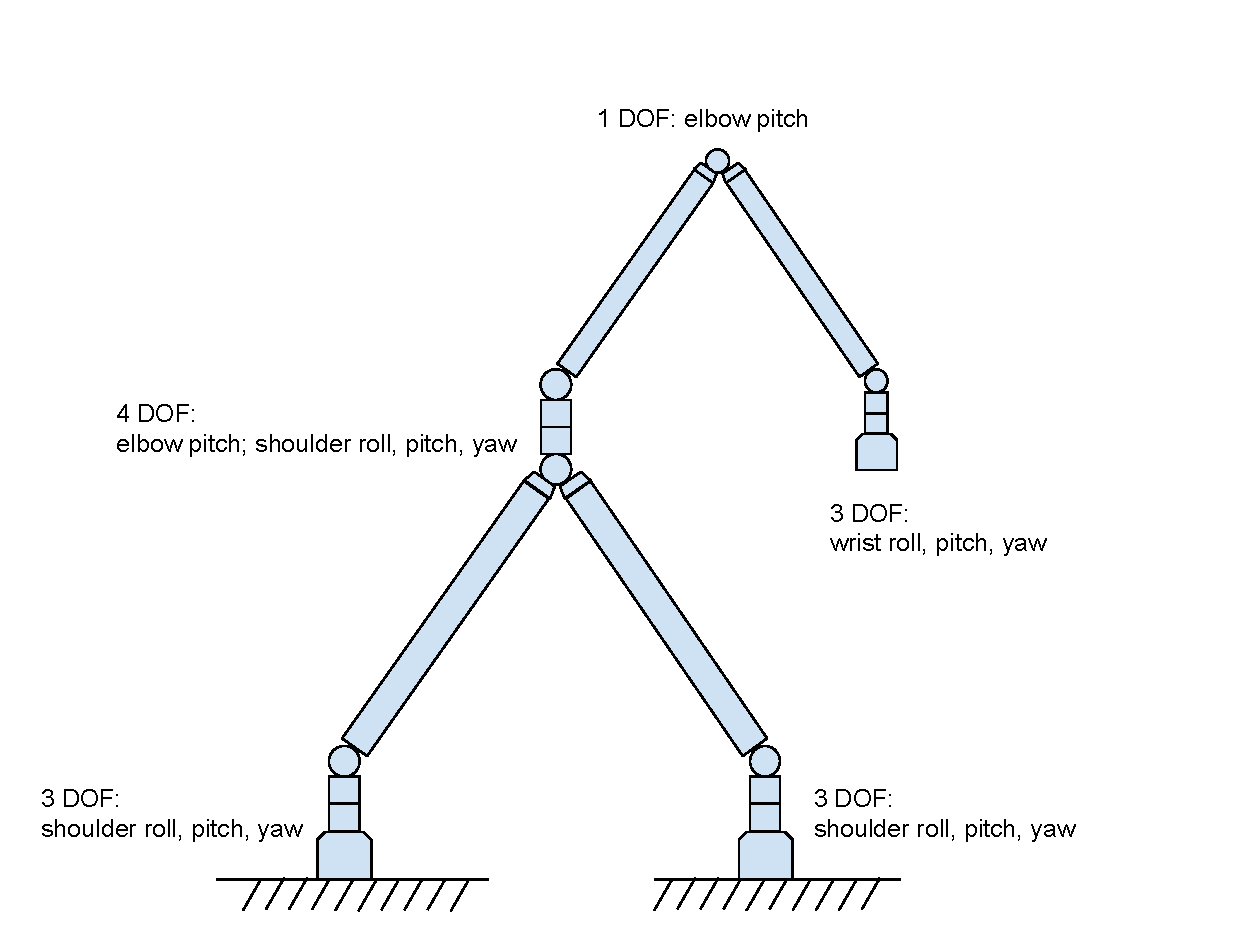
\includegraphics[width=0.5\textwidth]{14dof}
\caption{Sketch of 14DOF arm}
\label{fig:14dof}
\end{figure}
}
\item{\textbf{7 DOF robotic arm with 2 telescopic booms and 2 end effectors}\\
This architecture has two telescopic booms that would be extended once the robotic system is unstowed. The telescopic booms are extended by first connecting both end effectors on the Outpost and allowing the shoulder joint to freely rotate. Then, the elbow joint will rotate and extend the telescopic boom and two booms will extend separately.

The end effectors can grapple to Outpost to perform Outpost reconfiguration as well as free flying vehicles for capture and berthing. The end effectors can also connect to tools that are used for Outpost inspection and maintenance. The sketch of the architecture is shown in \Cref{fig:7dof} below.
\begin{figure}[H]
\centering
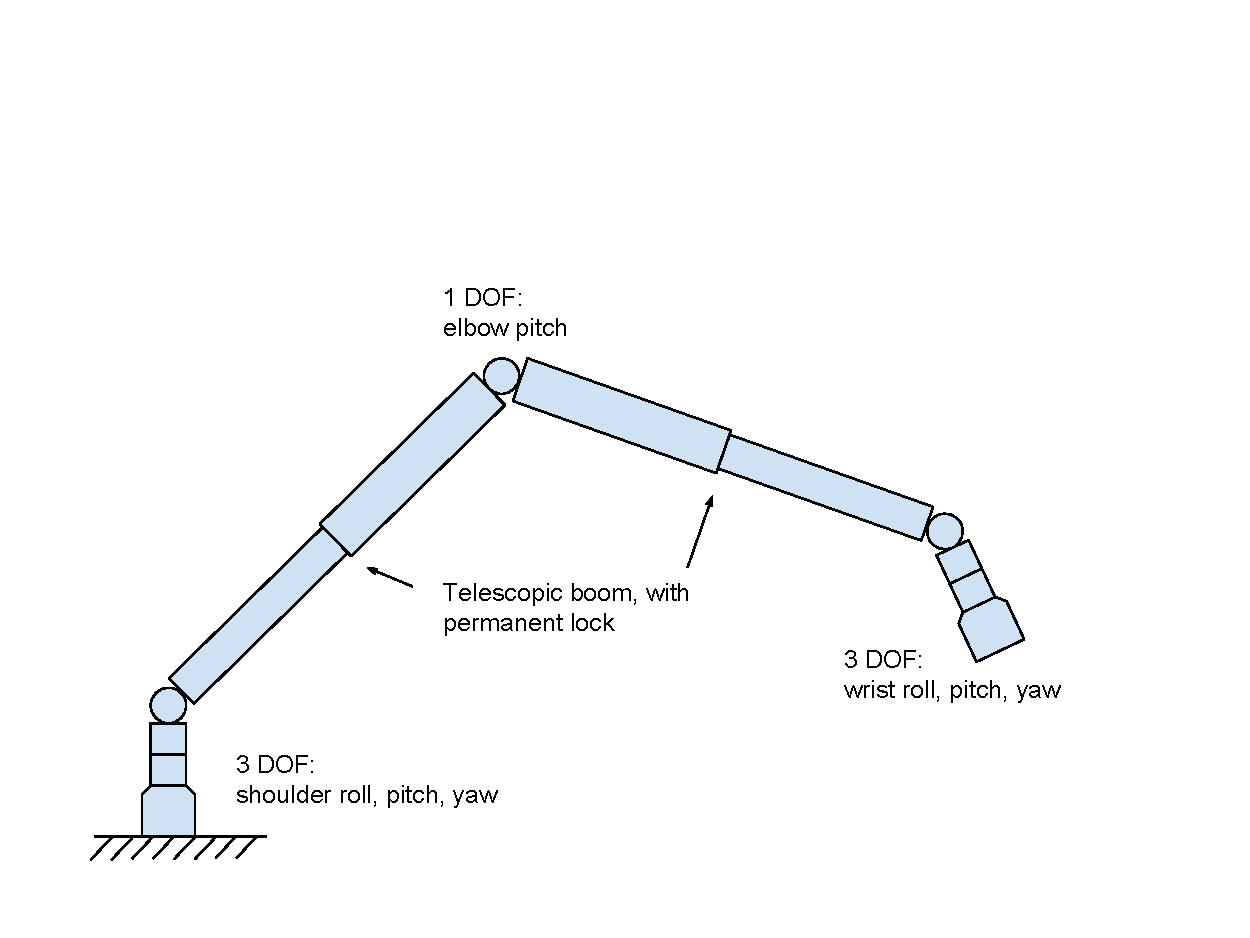
\includegraphics[width=0.55\textwidth]{7dof}
\caption{Sketch of 7DOF arm}
\label{fig:7dof}
\end{figure}
}
\item{\textbf{14 DOF robotic arm with truss rail, 2 booms and 2 end effectors}\\
As shown in \Cref{fig:14dof_truss} below, this design is composed of two parts. The first part is a 8 DOF arm with a truss rail and two booms. The end effectors can grapple to the Outpost to maneuver the robotic arm around the Outpost and perform Outpost reconfiguration. The end effectors can also grapple to free flyingr vehicles for capture and berthing operations. For inspection, maintenance and repair operations, two end effectors will be fixed on the Outpost and the truss rail between two elbow joints will act as guides for the fine arm.

The fine arm has 6 DOF and can move on the truss rail to perform inspection, maintenance and repair operations. Different tools can be attached to the end of the fine arm for specific tasks.
\begin{figure}[H]
\centering
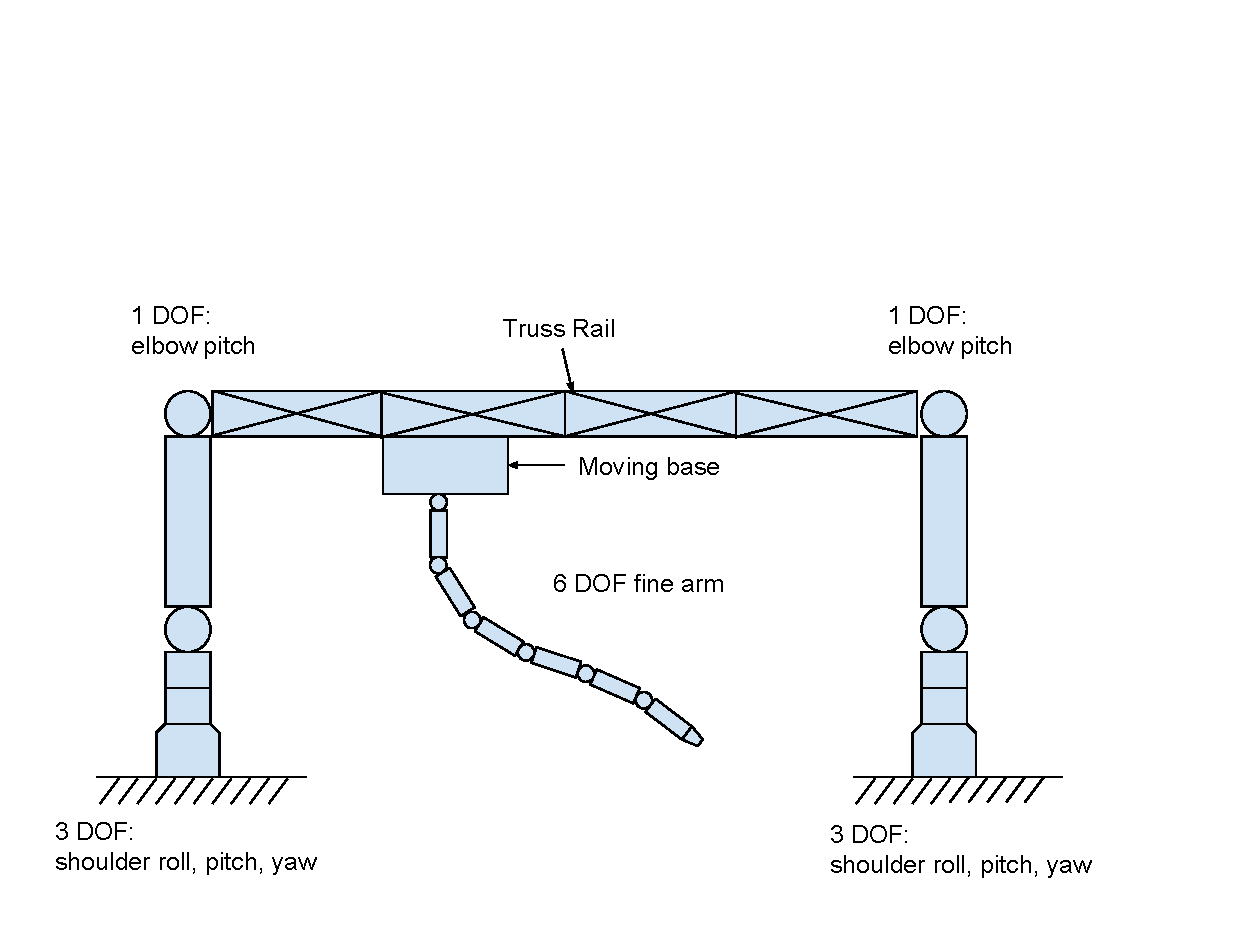
\includegraphics[width=0.6\textwidth]{14dof_truss}
\caption{Sketch of 14DOF arm with truss}
\label{fig:14dof_truss}
\end{figure}
}
\end{enumerate}

\begin{table}[H]
\centering
\caption{Trade Study of Architecture}
\begin{tabular}{|P{2.5cm}|P{4.1cm}|P{4.1cm}|P{4.0cm}|}
\hline
	&	\textbf{Architecture \#1}	&	\textbf{Architecture \#2}	&	\textbf{Architecture \#3}	\\\hhline{|=|=|=|=|}
\textbf{Structure Stability}	&
\textcolor{OliveGreen}{Robot has two fixed points on the Outpost, providing more stability}	&
\textcolor{red}{Robot has only one point fixed to the Outpost, arm will vibrate easily}	&
\textcolor{OliveGreen}{Robot has two fixed points on the Outpost, providing more stability}	\\\hline
\textbf{System Complexity}	&
\textcolor{red}{High complexity due to 14 degrees of freedom [Fund Robo]}	&
\textcolor{OliveGreen}{Lower complexity due to less degrees of freedom, heritage from Canadarm2}	&
\textcolor{red}{High complexity due to 14 degrees of freedom [Fund Robo]}	\\\hline
\textbf{Mass Required}	&
\textcolor{red}{Heaviest out of three due to 14 joints in total [That ERA thing]}	&
\textcolor{OliveGreen}{Lightest out of three\newline Least number of joints}	&
\textcolor{orange}{Medium: Has 8 joints and mechanical parts related to fine arm}	\\\hline
\textbf{Volume Occupied}	&
\textcolor{red}{Large volume due to more booms in the system}	&
\textcolor{OliveGreen}{Least volume out of three: 2 telescopic booms that are retracted in launch position}	&
\textcolor{red}{Large volume due to addition of truss and a fine arm}	\\\hline
\textbf{System Range}	&
\textcolor{orange}{Short range due to relatively shorter boom}	&
\textcolor{OliveGreen}{Long range due to telescopic boom that will extend}	&
\textcolor{orange}{Short range due to relatively shorter boom}	\\\hline
\textbf{Dexterous Tasks}	&
\textcolor{OliveGreen}{High stability due to smaller dexterous arm}	&
\textcolor{orange}{System can attach to tool for dexterous task\newline Low stability}	&
\textcolor{OliveGreen}{System has small dexterous arm\newline High stability}	\\\hline
\end{tabular}
\label{table:architectureto}
\end{table}

\subsection{Material of Frame}
\label{sect:materialto}
The material of the frame is directly related to the mass and shape of the system. Certain materials are too brittle to manufacture in desired shapes, and will affect the architecture of the system. As the material heavily affects mechanical aspects of the design, trade study on the material of frame was conducted. Material with low density, low coefficient of thermal expansion, and high strength are desired for the frame of the system. Commonly used materials in the space industry include carbon fiber, aluminum, stainless steel, and titanium. Each material has numerous variations with different properties and name. A trade study between four materials were conducted in table below.
\begin{table}[H]
\centering
\caption{Trade Study for type of Thermal Control System}
\begin{tabular}{|P{3.6cm}|P{3.1cm}|P{2.4cm}|P{2.3cm}|P{2.5cm}|}
\hline
	&	\textbf{PAN (Polyacrylonitrile) Carbon Fiber, Aerospace \cite{carbonfibreprop}}	&\textbf{Aluminium 7075 \cite{alumniumprop}}	&	\textbf{Stainless Steel 304 \cite{steelprop}}	&	\textbf{Titanium (Ti-6A/4V) \cite{titaniumprop}}	\\\hhline{|=|=|=|=|=|}
\textbf{Density (\si{\kilo\gram\per\metre\cubed})}	&	
1.8	&	2.81	&	8	&	4.43	\\\hline
\textbf{Ultimate Tensile Strength (\si{\mega\pascal})}	&
3450 to 5520	&	572	&	505	&	900 to 100	\\\hline
\textbf{Thermal Coefficient of Expansion (\si{\micro\metre\per\metre\per\kelvin})}	&	
-0.4 to -0.75	&	23.6	&	17.3	&	8.6	\\\hline
\textbf{Young's Modulus (\si{\giga\pascal})}	&
220 to 448	&	71.7	&	193 to 200	&	113.8	\\\hline
\end{tabular}
\label{table:materialto}
\end{table}

The specific properties of carbon fiber will vary with orientation and volume of the fibers and type of resin used. Aerospace grade carbon fiber, which has high stiffness to weight ratio, were selected for comparison. Other space robotic arms, such as Canadarm, Canadarm2, and ERA are made of carbon fiber as well. In general, carbon fiber is much lighter than titanium and stainless steel, have lower magnitude of thermal coefficient of expansion, and higher young’s modulus and tensile strength. Overall, aerospace grade carbon fiber is the most desirable option out of the four.

\subsection{Thermal Control System}
\label{sect:thermalto}
To ensure that temperatures of the subsystems are within their operating ranges, a thermal regulation system is required. In order to meet the requirement \textbf{TC-P-01}, which lists allowable temperature ranges, a trade study was conducted between active thermal control system (ATCS) and passive thermal control system (PTCS). ATCS makes use of various heaters and coolers to control the temperature within the system, and PTCS makes use of insulation to reduce heat transfer and surface coatings which modify the thermal or optical properties of the surface. The two types of thermal control system are compared in \Cref{table:thermalto}.
\begin{table}[H]
\centering
\caption{Trade Study for type of Thermal Control System}
\begin{tabular}{|P{2.5cm}|P{6.2cm}|P{6.2cm}|}
\hline
	&	\textbf{ACTS}	&	\textbf{PCTS}	\\\hhline{|=|=|=|}
\textbf{System Complexity}	&
\textcolor{red}{More complex due to electrical system and/or software in the system}	&
\textcolor{OliveGreen}{Less complex due to the lack of electrical system or software}	\\\hline
\textbf{System Reliability}	&
\textcolor{OliveGreen}{Can be manually controlled in the case of control system malfunction}\newline	\textcolor{OliveGreen}{Allows for more precise temperature control}\newline \textcolor{orange}{Needs repair if heating and cooling elements break down}	&
\textcolor{red}{No control system required for passive control}\newline \textcolor{orange}{Range of control is limited to materials}\newline \textcolor{OliveGreen}{More immune to failures due to lower complexity}	\\\hline
\textbf{System Efficiency}	&
\textcolor{orange}{Can be placed on standby mode to save power}	&
\textcolor{OliveGreen}{Limited power usage\newline Efficient in reducing heat transfer}	\\\hline
\textbf{Cost}	&
\textcolor{red}{Higher due to mechanical and electrical parts}	&
\textcolor{OliveGreen}{Lower as little or no installation required, no electrical or mechanical parts}	\\\hline
\textbf{Mass}	&
\textcolor{red}{Greater mass due to mechanical parts}	&
\textcolor{OliveGreen}{Lower mass, blankets and pain coatings weigh less than mechanical parts}\\\hline
\end{tabular}
\label{table:thermalto}
\end{table}
In \Cref{sect:materialto}, carbon fibre was selected as the frame material. Therefore, assuming the surface of the system is made of carbon fibre reinforced polymer, the expected surface temperature when it is fully exposed to sunlight is approximately 390 K. (\Cref{app:tempcalc}) The exact temperature will vary with fibre volume fraction, as well as type of the polymer. Although the maximum temperature is within the operational range of several components, it exceeds the operation range of sensitive components like electronics. Therefore, it is desirable to use multiple thermal systems to reduce the temperatures. Using only passive system and increasing redundancy does not improve the system reliability. Using only the active system and increasing the redundancy requires significant cost and mass. Therefore, it is decided that the system will use combination of active and passive thermal control system for efficient temperature control. Further calculation shows that coating the surface with white paint reduces the absorptivity/emissivity ratio and reduces the expected surface temperature further.

\subsection{Power Storage}
\label{sect:powerto}
In order to provide the robotic system with power to run during contingencies, a power storage subsystem is required. A trade study of the two most commonly used rechargeable batteries in space, Li-ion and NiH$_2$ batteries,
 is conducted in \Cref{table:powerto}.
\begin{table}[H]
\centering
\caption{Trade Study for type of Power Storage}
\begin{tabular}{|P{6cm}|P{4.2cm}|P{4.2cm}|}
\hline
	&	\textbf{Li-ion}	&	\textbf{Ni-H}	\\\hhline{|=|=|=|}
\textbf{Used in}	&
Mars Rovers: Spirit \& Opportunity \cite{Liion_Mars}	&
International Space Station \cite{ISS_power}	\\\hline
\textbf{Specific Energy (Wh/kg)}	&
150 \cite{batt_primer}	&	65 \cite{NiH_se}	\\\hline
\textbf{Energy Density (Wh/L)}	&
400 \cite{batt_primer}	&	10-80 \cite{NASA_energy}	\\\hline
\textbf{Cycle Durability}	&
1000 \cite{batt_primer}	&	\textgreater50000 \cite{NASA_energy}	\\\hline
\textbf{Operable Temperature (\si{\degreeCelsius})}	&
-20 to 60 \cite{batt_primer}	&	-5 to 30 \cite{NASA_energy}	\\\hline
\textbf{Lifespan (years)}	&
\textgreater2 \cite{NASA_energy}	&	\textgreater10 \cite{NASA_energy}	\\\hline
\end{tabular}
\label{table:powerto}
\end{table}
Li-ion batteries are able to provide much more energy with a smaller mass and volume than NiH$_2$ batteries. Li-ion batteries are also operable over a much larger temperature range than NiH$_2$ batteries. Although Li-ion batteries can endure much less charge cycles than NiH$_2$, this would not be a huge problem as the batteries will only be used in contingencies, and will not be subjected to discharging and recharging on a frequent basis. The most major drawback related to the use of Li-ion batteries is the short life span, which would mean that it has to be replaced fairly frequently.

\subsection{End Effector}
\label{sect:endeffectorto}
In order to interact with the external subsystems situated around EML2, including the Outpost, astronauts and other modules during various operations, an end effector subsystem is required to build connections with the Outpost and other modules. And the interface established by the end effector shall capable of providing power and data connections to and from the robotic system.

As a result of those criteria, two potential end effector models are listed and compared below:

\textbf{Three fingers-three petals End Effector}: There are two main subassemblies of this end effector: an active mechanism, which consists of a motor driven lead screw that would accurate the linkages between the three finger and three petals; a passive structure, whose geometry will allow it to be constrained by the linkages and therefore establishing a rigid interface.	\\
\textbf{Steel cable-snared End Effector}: This end effector system consists of the snaring and rigidizing subassembly inside the shell, and four latch/umbilical subassemblies outside the shell, which are responsible for the rigidizing loop and the connecting loop after the fine positioning for latching and connecting operation is reached.
\begin{table}[H]
\caption{Trade Study for type of End Effector}
\begin{tabular}{|P{2.5cm}|P{6.35cm}|P{6.35cm}|}
\hline
	&
\textbf{Three fingers-three petals End Effector}	&
\textbf{Steel cable-snared End Effector}	\\\hhline{|=|=|=|}
\textbf{System Complexity}	&
\textcolor{OliveGreen}{Two main subassemblies\newline Can accomplish capturing, rigidizing and connection by only one actuator. \cite{CJME_EE}}	&
\textcolor{OliveGreen}{Two main subassemblies\newline An orbit replaceable unit, end effector can be easily replaced or repaired on orbit \cite{CJME_EE}}	\\\hline
\textbf{Operation Accuracy}	&
\textcolor{OliveGreen}{Capable of misalignment tolerance}\newline\textcolor{red}{Not suitable for soft capture \cite{CJME_EE}}	&
\textcolor{OliveGreen}{Has a strong capability of misalignment tolerance\newline Has enormous capability of soft capture \cite{CJME_EE}}	\\\hline
\textbf{Mass Required}	&
\textcolor{orange}{Maximum \SI{50}{\kilo\gram} \cite{orbital_capture}}	&
\textcolor{orange}{Maximum \SI{50}{\kilo\gram} \cite{orbital_capture}}	\\\hline
\textbf{Volume Occupied}	&
\textcolor{red}{Relatively large: maximum circumradius \SI{350}{\milli\metre} to \SI{500}{\milli\metre} \cite{CJME_EE}\cite{orbital_capture}}	&
\textcolor{OliveGreen}{Small: maximum circumradius \SI{280}{\milli\metre} \cite{CJME_EE}}	\\\hline
\textbf{Power Required}	&
\textcolor{OliveGreen}{Low, only one actuator required \cite{CJME_EE}}	&
\textcolor{OliveGreen}{Low, maximum \SI{100}{\watt} \cite{ERA_EE}}	\\\hline
\textbf{Maximum Payload}	&
\textcolor{red}{Relatively small \cite{orbital_capture}}	&
\textcolor{orange}{Large at a low speed \cite{ERA_EE}}	\\\hline
\end{tabular}
\label{table:endeffector}
\end{table}
According to this comparison, the second design - Steel cable-snared End Effector is more suitable for our project. And in addition to those advantages listed, the Steel cable-snared End Effector is a proven technology, which has been applied on existing projects like the European Robotic Arm (ERA).

\subsection{Locomotion - Motor type}
\label{motorto}
In order to efficiently navigate around the Outpost and move astronauts as well as other modules to their desired destination, a proper types of motors need to be selected for the locomotion subsystem. The chosen motor shall be able to fit in the mass/volume constraints, and shall capable of providing enough torque to the system. Three models have been considered – Stepper Motor, Brushless DC Motor and Brush DC Motor, which are compared in \Cref{table:motorto}:

\begin{table}[H]
\caption{Trade Study for Type of Motor}
\begin{tabular}{|P{2.5cm}|P{4.1cm}|P{4.1cm}|P{4.1cm}|}
\hline
	&
\textbf{Stepper Motor}	&	
\textbf{Brushless DC Motor}	&
\textbf{Brush DC Motor}	\\\hhline{|=|=|=|=|}
\textbf{Torque Capability}	&
\textcolor{orange}{High torque/power ratio at low speed and low power \cite{ESA_motor}}\newline\textcolor{red}{Short term-peak torque capability is limited by magnetic saturation\newline Low angular torque stiffness\newline  Noisy, creating significant speed ripple and microgravity disturbances \cite{ESA_motor}}	&
\textcolor{OliveGreen}{Torque/power is  high\newline Given torque can be obtained at any working speed, if power allows\newline Significant short-term peak torque capability, with a peak value which can be more than five times the nominal demand\newline Less noise\cite{ESA_motor}}	& 
\textcolor{OliveGreen}{Similar to the Brushless DC Motor, with lower power consumption \cite{ESA_motor}}\newline\textcolor{red}{Brushes have major drawbacks in space environments (i.e. disruptive voltages after a dormant period) \cite{ESA_motor}}   \\\hline
\textbf{Electric Driver Complexity}	&
\textcolor{OliveGreen}{Simplest\newline Resulting incremental stepping motion matches with many mechanisms requirements \cite{ESA_motor}}	&
\textcolor{red}{More complex than “simplest” stepper motor driver \cite{ESA_motor}}\newline\textcolor{orange}{Complexity will be reduced if a position exists in system  \cite{ESA_motor}}  & 
\textcolor{red}{Similar to the brushless DC motor \cite{ESA_motor}} 	\\\hline
\textbf{Mass/ Volume Required}	&
\textcolor{OliveGreen}{Usually does not require a dedicated position sensor \cite{ESA_motor}}	&
\textcolor{red}{Always needs a position sensor \cite{ESA_motor}}   & 
\textcolor{OliveGreen}{Mass/size is relatively smaller than brushless DC Motor\cite{ESA_motor}}	\\\hline
\end{tabular}
\label{table:motorto}
\end{table}
From the trade study, the brushless DC motor has a better performance than the other two compared models, and has a significant advantage at the torque capability. Also, brushless DC motor has been considered for previous space arm robot project \cite{ERA_motor}, which will decrease its development risk. Therefore, a brushless DC motor is chosen to be used on the locomotion subsystem.

\subsection{Locomotion - Joint type}
\label{sect:jointto}
As a major part of the locomotion subsystem, the joints utilize rotation of the motors to accomplish the motion of robotic arm. Two different joint structures that used in reference designs are inline joint and offset joint. Inline joint is used in European Robotic Arm and offset joint is used in Canadarm2. Depend on the tasks that two arms need to perform, both joint structures have advantages and disadvantages.
\begin{table}[H]
\caption{Trade Study for type of Joint}
\begin{tabular}{|P{2.5cm}|P{6.35cm}|P{6.35cm}|}
\hline
	&	\textbf{Inline Joint}	&
	\textbf{Offset Joint}	\\\hhline{|=|=|=|}
\textbf{Operation Complexity}	&
\textcolor{OliveGreen}{No joint collision risk, components are in the same plane.}	&
\textcolor{red}{Add complexity to task due to possibility of joint collision [comp]}	\\\hline
\textbf{Operation Range}	&
\textcolor{red}{Limited mobility; limited motor rotational range.}	&
\textcolor{OliveGreen}{The arm can maneuver more readily over large areas by “stepping over the elbow”; large motor rotational range[comp]}	\\\hline
\end{tabular}
\label{table:jointto}
\end{table}

The major task for Canadarm2 was to assemble the ISS. By having offset joints, the joint can rotate in larger range and enable the arm to have more flexible motion. \Cref{table:jointrange} in \Cref{app:jointrange} shows the joint motion range for Canadarm2 and ERA \cite{arm_comp}. As the robotic system on the Outpost needs to perform reconfiguration operation, it is important to have large range of motion to maneuver the Outpost module. Therefore the offset joint structure is chosen for the locomotion subsystem.

%--------------------------------------------------------------------------------------------------------------------------------------------------------------------------------
\section{Architecture}
\label{sect:architecture}
The physical architecture of the robotic system is displayed in the figure below. The architecture is designed from the trade-offs discussed: the system will have 7 DOF, 2 telescopic carbon fiber booms. The number of DOF and material of the frame were derived from \Cref{sect:architectureto,sect:materialto} respectively. Telescoping booms increases the reach of the system at the cost of an increase in mass compared to a boom of similar length.

\Cref{fig:stowedarm,fig:openedarm} shows the system in stowed and deployed configurations respectively.Three joints (red) and sensor units (green) are placed at the end of the booms, and power unit (purple) and data handling unit (yellow) are placed on the middle joint. End effector subsystem (orange) is located at the end of each arm, and sensors are located at each joints to obtain thermal, mechanical, and visual data. Finally, thermal control subsystem is located inside the frame (white) and cables and distribution channels connecting subsystems are placed inside the frame.

\begin{figure}[H]
\centering
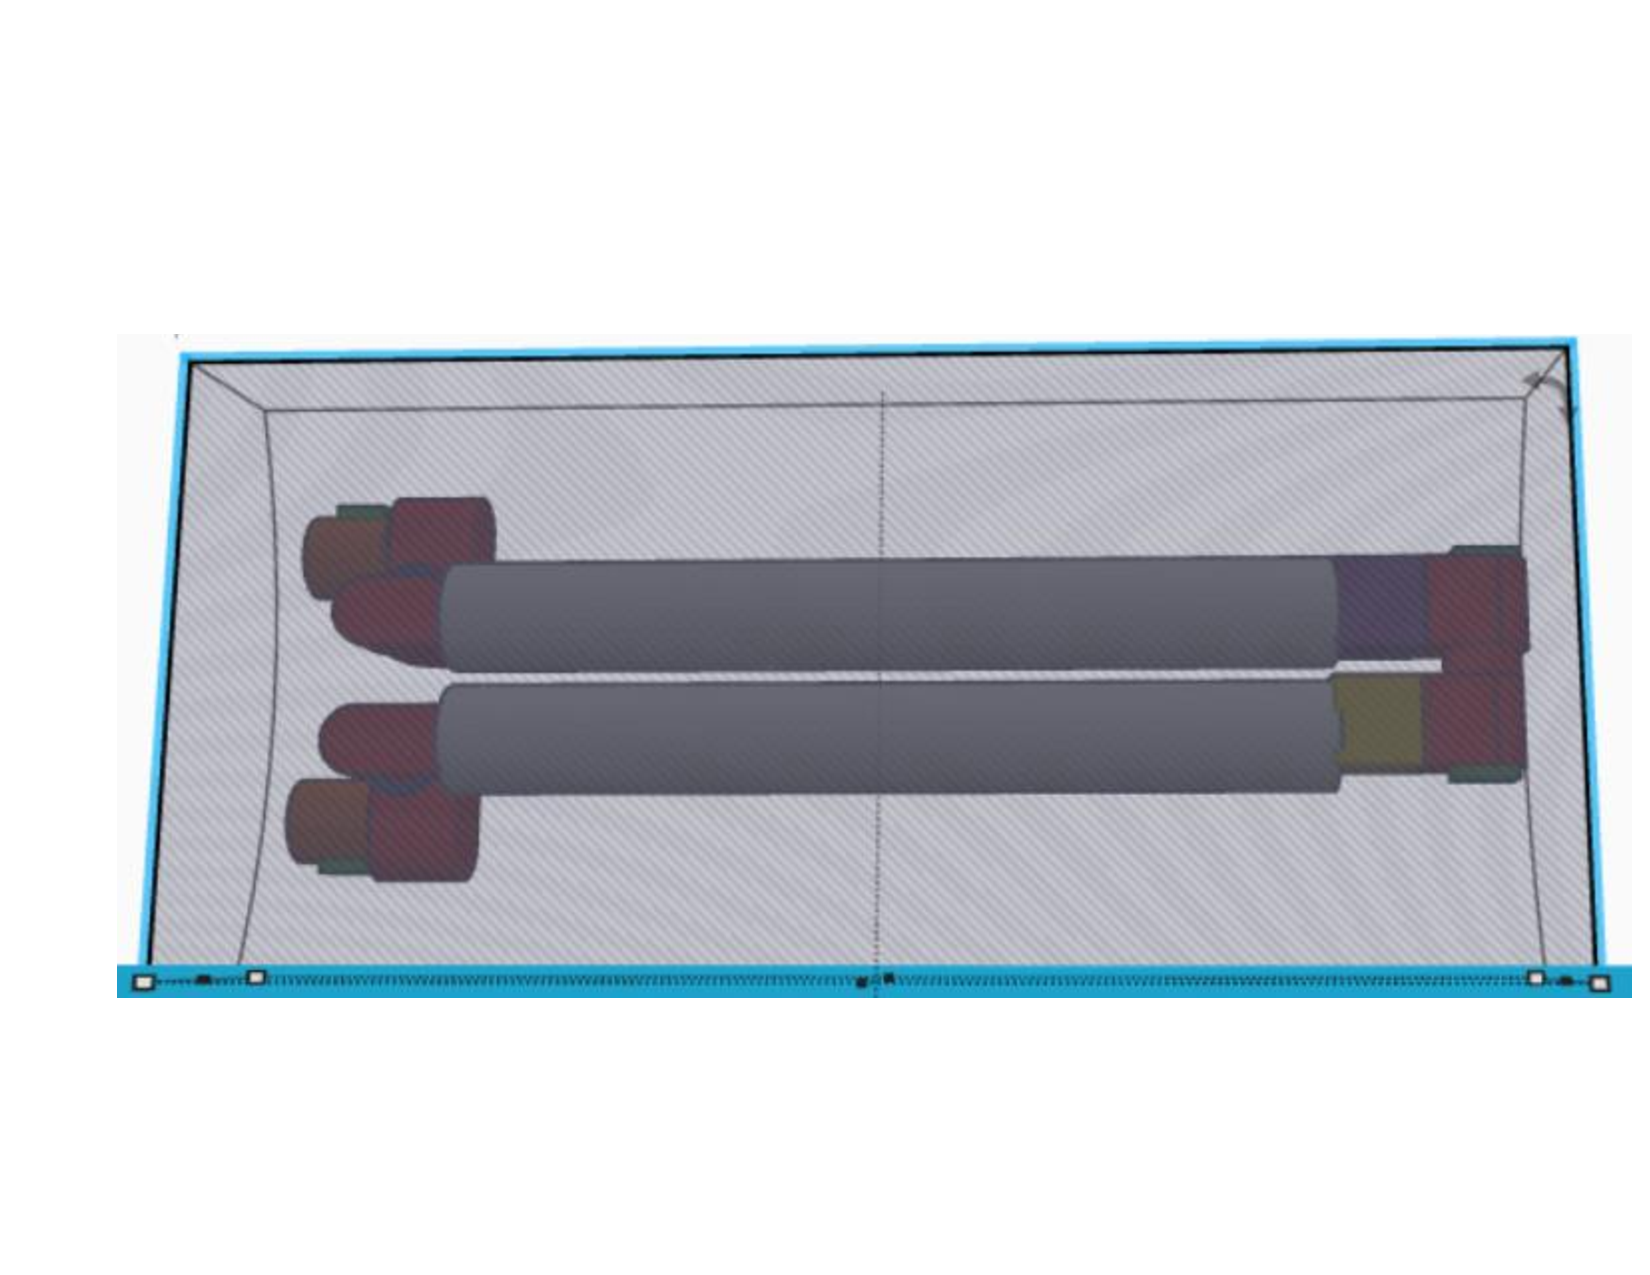
\includegraphics[width=0.8\textwidth]{stowedarm}
\caption{Robotic System in stowed configuration}
\label{fig:stowedarm}
\end{figure}

\begin{figure}[H]
\centering
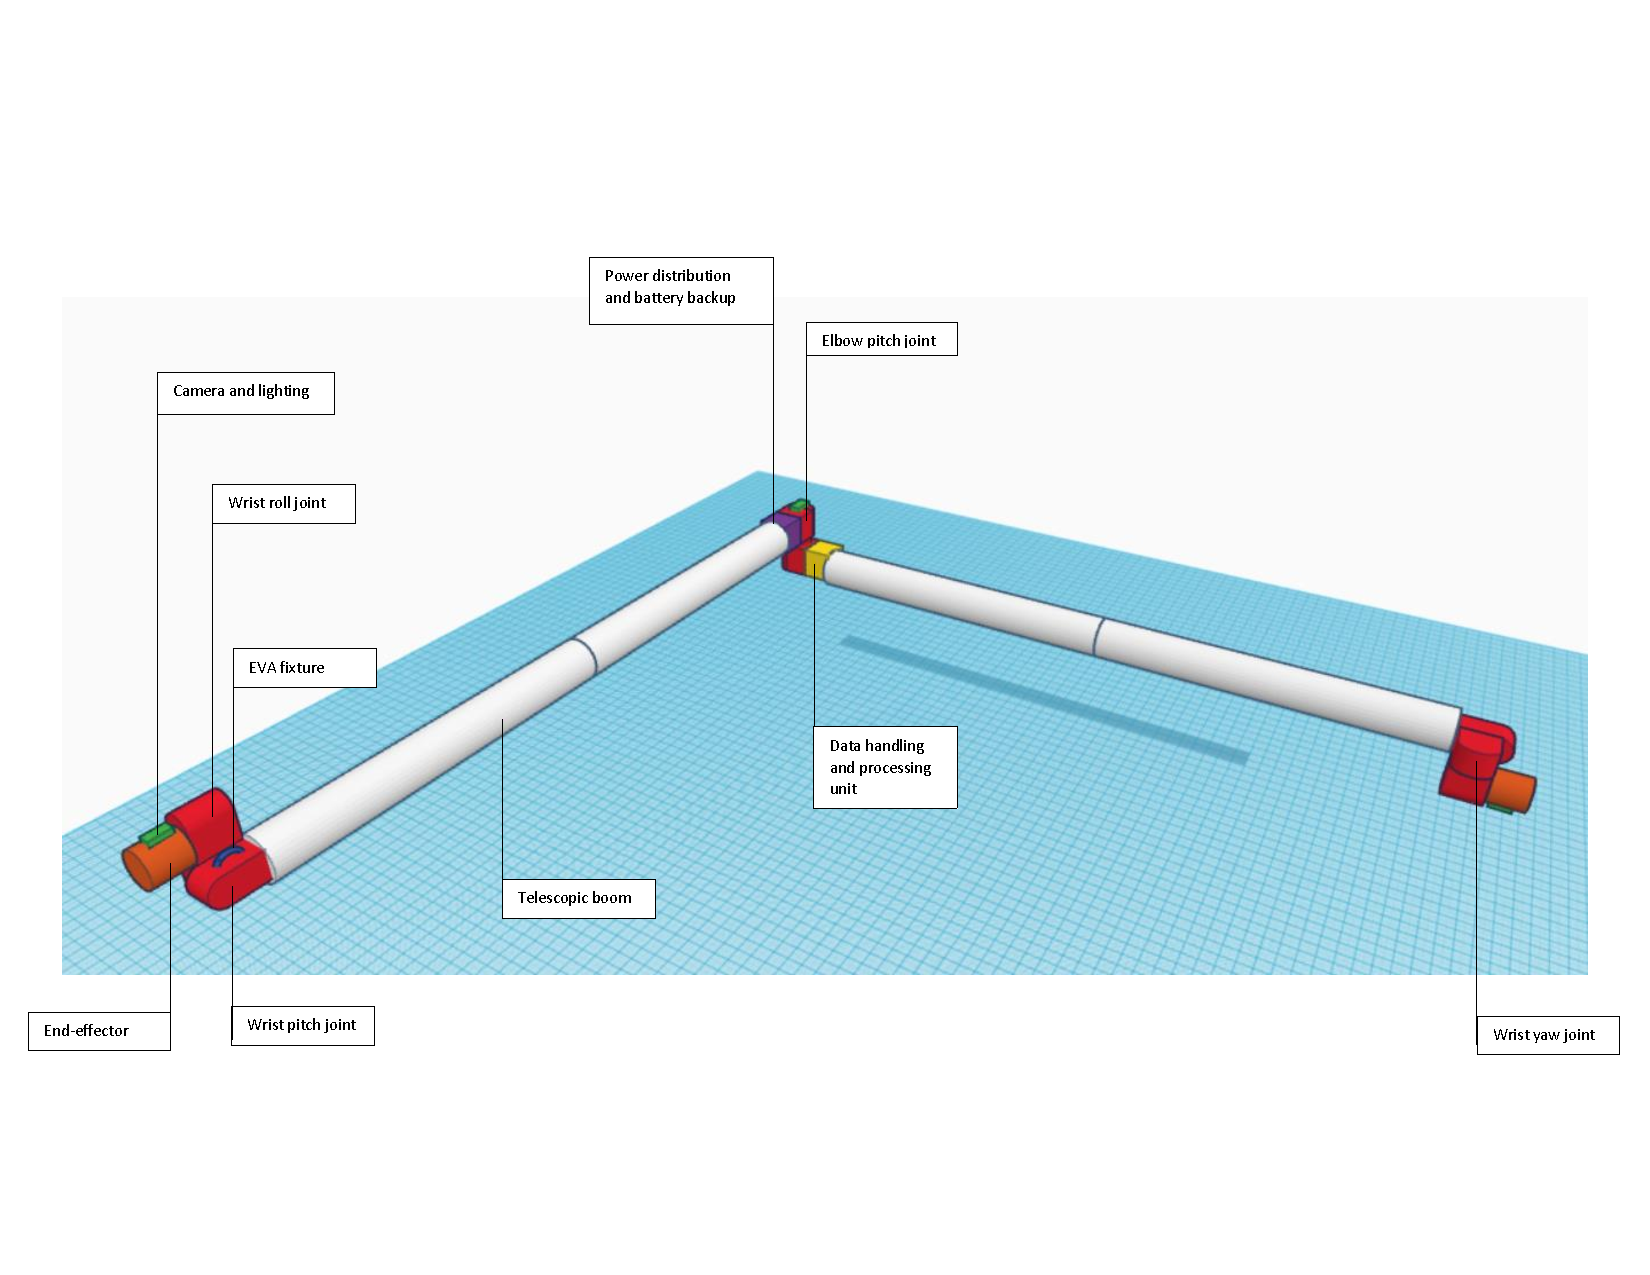
\includegraphics[width=\textwidth]{openedarm}
\caption{Robotic System in deployed configuration}
\label{fig:openedarm}
\end{figure}
%--------------------------------------------------------------------------------------------------------------------------------------------------------------------------------
\section{Mass Budget}
\label{sect:mass}
\Cref{table:mass} outlines the estimated mass budget for each of the subsystems. The estimates are justified below.

\begin{table}[H]
\centering
\caption{Mass Budget}
\begin{tabular}{cccc}
\toprule
\textbf{Subsystem}	&	\textbf{Mass(kg)}	&	\textbf{Percentage}	&	\textbf{Margin}\\\midrule
\textbf{Locomotion}						&	141.75	&	45\%&	30\%\\
\textbf{Data Handling \& Processing}	&	15.75	&	5\%	&	30\%\\
\textbf{Thermal Control}				&	12.6	&	4\%	&	30\%\\
\textbf{Power}							&	6.3		&	2\%	&	30\%\\
\textbf{End Effector}					&	69.3	&	22\%&	30\%\\
\textbf{Sensors}						&	6.3		&	2\%	&	30\%\\
\textbf{Frame}							&	31.5	&	10\%&	30\%\\
\textbf{Cables}							&	31.5	&	10\%&	30\%\\\hline
\textbf{Total}	&	\textbf{315}	&	\textbf{100\%}	&	\textbf{30\%}	\\\bottomrule
\end{tabular}
\label{table:mass}
\end{table}

\textbf{Total Mass}: Mass constraint of \SI{450}{\kilo\gram} \cite{RFP}, and mass margin is 30\%.

\textbf{Locomotion}: Based in ERA joint percentages \cite{ERA_joints}, adjusted as electronics and cabling are accounted for separately. 

\textbf{Data Handling \& Processing}: The appropriate mass percentage for this subsystem was determined based on the design of other space systems and their mass breakdowns. \cite{LISA_budget, TUD_mass, NASA_microrover}

\textbf{Thermal Control}: The passive thermal control components are extremely lightweight, and based on other space system designs \cite{TUD_mass}, it was determined that the thermal control subsystem will account for a relatively low portion of the mass budget.

\textbf{Power}: Batteries should not weigh less than \SI{6.3}{\kilo\gram}, especially for the purpose of this robotic system as an emergency, temporary power source. (\Cref{sect:power})

\textbf{End Effector}: Typical end effectors weigh a maximum of \SI{50}{\kilo\gram}, including cabling, cameras, and electrical equipment. (\Cref{sect:endeffector})

\textbf{Sensors}: Cameras and lighting fixtures for inspection account for the majority of the weight for this subsystem. These components typically weigh about \SI{500}{\gram} to \SI{1}{\kilo\gram}, whereas other sensors are relatively insignificant in terms of mass.  \cite{cameras}

\textbf{Frame}: Using designs for a telescopic boom \cite{ESM_telescopic}, and referencing Canadarm \cite{IEEE_Carm}, it was determined that the booms will weigh about \SI{15}{\kilo\gram} to \SI{20}{\kilo\gram} each.

\textbf{Cables}: The mass of cabling is typically about 10\% of the total system mass for manipulators for systems similar to the Canadarm \cite{IEEE_RMSperformance}.

\section{Conclusion}
\label{sect:conclusion}


%--------------------------------------------------------------------------------------------------------------------------------------------------------------------------------
\newpage
\bibliographystyle{unsrt}
\bibliography{reportbib}

\newpage
\appendix
\section{Temperature Range of Components}
\label{app:optemp}
\begin{table}[H]
\caption[Operational and Survival Temperature Ranges of various Components]{Operational and Survival Temperature Ranges of various Components \cite{NASAsysreq_Kumar}}
\centering
\begin{tabular}{|l|l|l|}
\hline
\textbf{Component}	&	\textbf{Operational (\si{\degreeCelsius})}	&	\textbf{Survival (\si{\degreeCelsius})}\\\hhline{|=|=|=|}
\textbf{Gears \& Bearings}		&	-25 to 135	&	-50 to 155	\\\hline
\textbf{Motor Windings}			&	-25 to 180	&	-50 to 200	\\\hline
\textbf{Brakes}					&	-25 to 99	&	-50 to 120	\\\hline
\textbf{Cables \& Connectors}	&	-70 to 135	&	-90 to 155	\\\hline
\textbf{Electronics}			&	-20 to 65	&	-50 to 85	\\\hline
\end{tabular}
\end{table}

\subsection*{Data from External Documents}
\begin{figure}[H]
\centering
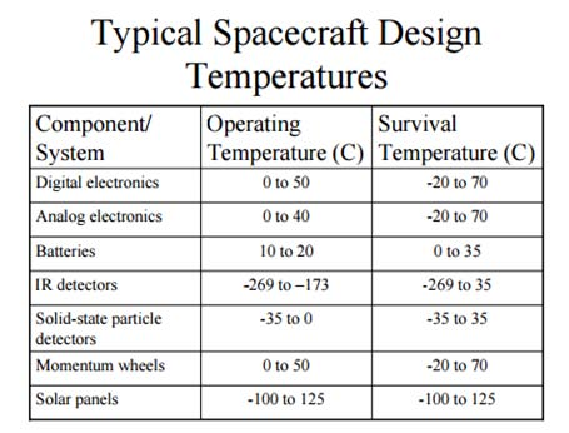
\includegraphics[scale=0.6]{Apppic/designtemp}
\caption[Typical Spacecraft Design Temperatures]{Typical Spacecraft Design Temperatures \cite{spacedesigntemp}}
\end{figure}
\begin{figure}[H]
\centering
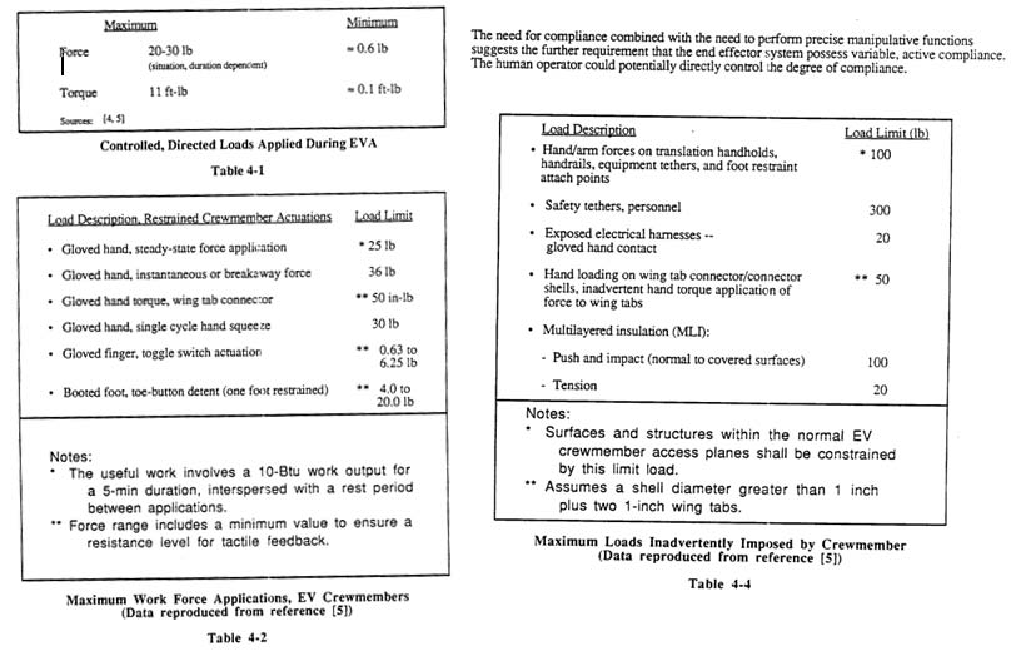
\includegraphics[scale=0.6]{Apppic/eeloads}
\caption[End Effector Load Limits]{End Effector Load Limits \cite{NASAEE_Mishkin}}
\end{figure}
\begin{figure}[H]
\centering
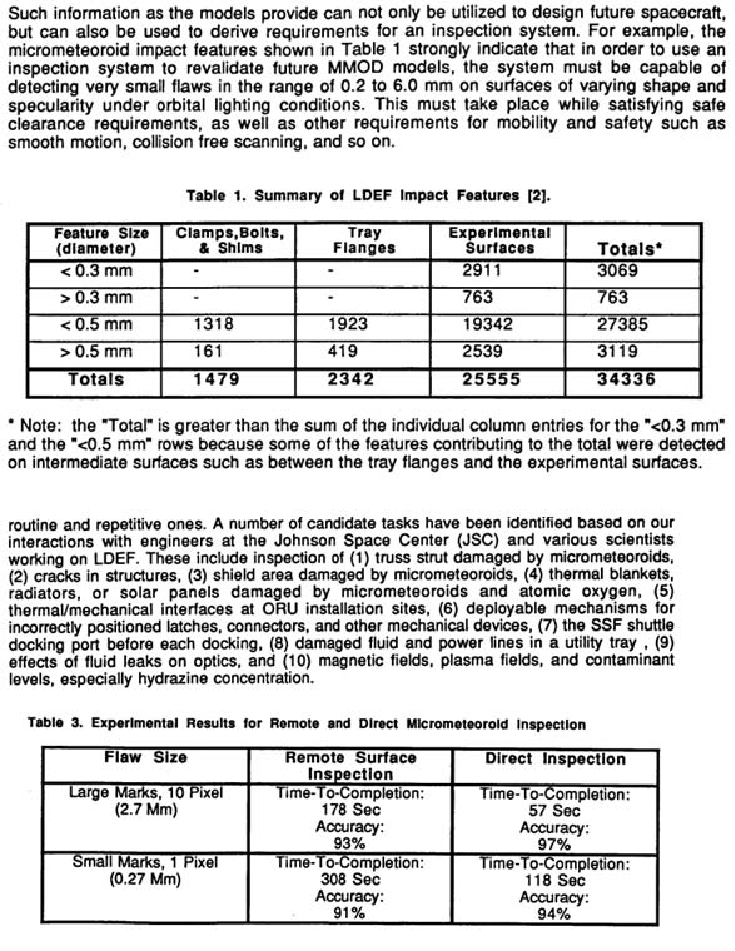
\includegraphics[scale=1]{Apppic/inspect}
\caption[Requirements for Inspection Systems]{Requirements for Inspection Systems \cite{NASAinspect_Hayati}}
\end{figure}
\section{Thermal Calculations}
\label{app:tempcalc}
\setcounter{equation}{0}
This calculation shows expected surface temperature of the system when it is fully exposed to the sunlight.

The thermal equation can be expressed as:
\begin{equation} 
q_{absorbed}+q_{internal} = q_{radiation}
\end{equation}
\begin{equation} 
q_{radiation}=e\times A\times\sigma \times T^{4}
\end{equation}
\begin{equation} 
q_{absorbed}=a\times A\times q_{sun}
\end{equation}
Due to lack of atmosphere, there is little heat transfer by conduction and convection. Assuming the sun is the primary source of absorbed heat and the system is located in EML2, albedo and emission, which are caused by radiation from earth or reflection from the earth, were considered insignificant.
\begin{equation}
q_{absorbed}=q_{radiation}
\end{equation}
\begin{equation}
a\times A\times q_{sun}=e\times A\times\sigma \times T^{4}
\end{equation}
where: \\
$e$: Emissivity\\
$A$: Surface Area \\
$\sigma$: Stefan-Boltzmann Constant \\
$T$: Surface Temperature \\
$a$: Absorptivity \\
$q_{sun}$: Solar Irradiance \\


Based on the trade studies, carbon fiber is selected as the surface material, which has emissivity and absorptivity of approximately 0.85. EML2 is approximately 1 astronomical unit away from the Sun. Assuming the system is fully exposed to sunlight at EML2, the solar irradiance is expected to be approximately \SI{1360}{\watt\per\square\metre}\cite{IM_solidprop}\cite{GPL_solar}.

Substituting the variables in the equation, the temperature of the surface can be calculated:
\begin{center}
$T_{surface} =(\frac{a\times q_{sun}}{e\times \sigma})^{\frac{1}{4}}$ \\
$T_{surface} = 394 K$
\end{center}
Carbon fiber has absorptance/emissivity ratio of approximately 1. White paint coatings, such as Zerlauts White Paint and Hughson White Paint, have much lower ratio. Using \textit{Hughson White Paint Z-202+1000} as an example, which has absorptivity of 0.4 and emissivity of 0.87, the expected surface temperature decreases by \SI{70}{\kelvin} to approximately \SI{324}{\kelvin} \cite{RRE_solar}. 
\section{Load Calculations}
\label{app:loadcalc}
\setcounter{equation}{0}
At EML2, the gravitational acceleration is nearly zero, the force acting on the arm is coming from external contact like EVA or the acceleration of payload.

\large \textbf{Payload reaction force/torque}\\
\normalsize There is no moving speed and stopping distance requirement proposed by customer. However, we can use the performance of reference design such as Canadarm and Canadarm2 to calculate a reference loading requirement. 

Tip velocity of Canadarm with full payload:$v=0.06m/s$\\
Canadarm stopping distance with full payload: $b=0.6m$\\
Leaving a 30\% margin, Stopping Distance: $b=0.42m$\\
Maximum payload mass from RFP: $m=10000kg$

Assume payload acceleration is constant, the following two equations are used to calculate acceleration:
\begin{equation}
b=v_it+\frac{1}{2}at^2
\end{equation}
\begin{equation}
a=\frac{v_f-v_i}{t}
\end{equation}
where:\\
$v_i=v$ is the initial velocity of payload\\
$v_f=0$ is the final velocity of payload\\
This gives us a result of $$t=14s, a=0.0043m/s^2$$

The reaction force applied by the payload is 
$$F=ma=10000kg\times0.0043m/s^2=43N$$

This reaction force will apply a bending moment to the robotic arm. Another type of load applied by the payload is torque due to the rotational motion. Canadarm2's rotational velocity and stopping angle are used. 

Rotational Velocity: $\omega=0.24\deg/s=0.0042rad/s$ \cite{NASAsysreq_Kumar}\\
Rotational Stopping Distance: $\theta=3.8\deg$
Leaving a 30\% margin, Stopping Distance: $\theta=2.9\deg=0.051rad$

These two performance characteristics of Canadarm2 are associated with payload that has mass of \SI{209000}{\kilo\gram} and size of \SI{4.5}{\metre} in diameter and \SI{17}{\metre} in length. This mass is twice of the maximum required in RFP and the size of the payload was not specified in the RFP. The size of the payload handled by the robotic system is assumed half the length of Canadarm2 payload. This size is also a close resemblance of a service module on ISS \cite{ISS_Harmony}.

Maximum payload mass from RFP: $m=10000kg$
Payload size: diameter $d=4.5 m$; length $l=8.5 m$
Assume payload has uniform density, payload moment of inertia:
$$I=\frac{1}{4}m(\frac{d}{2})^2+\frac{1}{2}ml^2=253490 kg\cdot m^2$$
The axis for the moment of inertia is chosen according to the location of the grapple fixture on the ISS module\cite{ISS_Harmony}. The axis is marked as a black dotted line in \Cref{fig:harmony_axis}.

\begin{figure}[H]
\centering
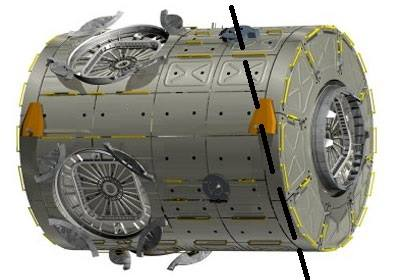
\includegraphics[width=0.4\textwidth]{Apppic/harmony}
\caption{Axis used to calculate moment of inertia}
\label{fig:harmony_axis}
\end{figure}

Assuming payload rotational acceleration is constant, the following two equations are used to calculate rotational acceleration.
\begin{equation}
\theta=\omega_it+\frac{1}{2}\alpha t^2
\end{equation}
\begin{equation}
\alpha=\frac{(\omega_f-\omega_i)}{t}
\end{equation}
where:\\
$\omega_i=\omega$ is the initial rotational velocity of payload\\
$\omega_f=0$ is the final rotational velocity of payload

This gives us the result of $$t=24s, \alpha=0.00177rad/s^2$$
The reaction torque applied by the payload is then
$$\tau=I\alpha=253490kg\cdot m^2\times 0.00177rad/s^2=448.7Nm$$

\large \textbf{Holding/Reaction forces}\\
\normalsize Requirement \textbf{EE-P-02} states that the end effector subsystem shall apply holding or reaction forces of \SI{200}{\newton} in any direction.

\large \textbf{Holding/Reaction forces}\\
\normalsize The robotic arm can be modeled as a cantilever beam and the highest load occurs when the arm is straight as shown in \Cref{fig:loading} below. The holding and reaction force is higher than the payload reaction force, therefore the force of \SI{200}{\newton} from holding and reaction is used.

\begin{figure}[H]
\centering
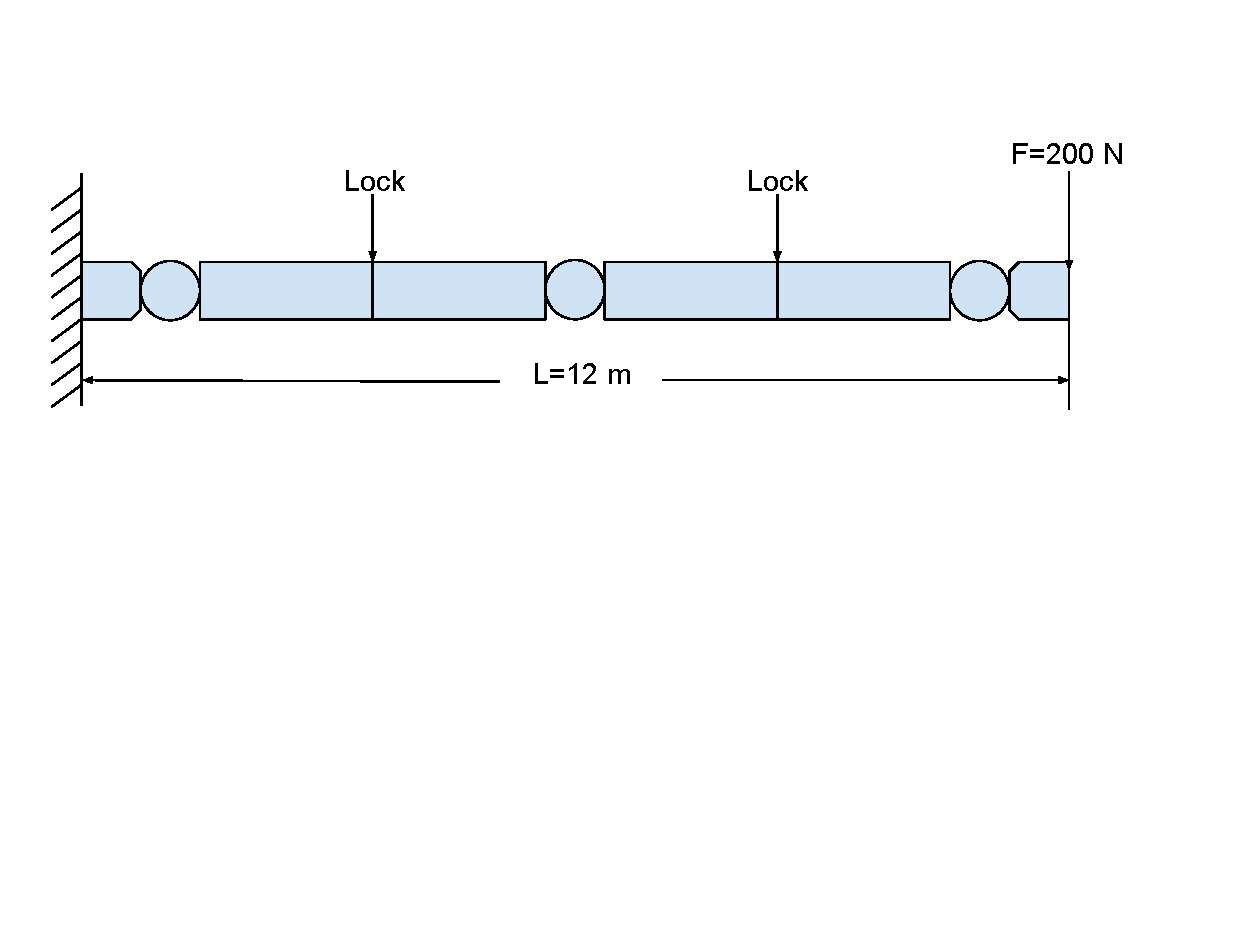
\includegraphics[width=0.6\textwidth]{Apppic/loading}
\caption{Maximum loading configuration of system}
\label{fig:loading}
\end{figure}

The maximum moment is at the end effector and shoulder joint.
$$M=FL=2400Nm$$
The moment at the lock where the telescopic boom is locked is:
$$M_{Lock} = FL_{Lock} = 1800 Nm$$
The moment at the elbow joint is:
$$M_{elbow} = FL_{elbow} = 1200 Nm$$
Given factor of safety of 1.5, the final bending moments on the arm are:
$$M =3600 Nm, M_{Lock} =2700 Nm, M_{elbow} =1800 Nm$$
The rotational torque load on the arm is:
$$T = 448.7 Nm\cdot1.5=673.05 Nm$$

\large \textbf{Other reference load requirement}\\
\normalsize \textbf{End Effector}\\
The end effectors of Canadarm2 need to perform snare, rigidize and latch mechanism, the load transfer capability of the end effector are \cite{NASAsysreq_Kumar}:\\
i) ``\SI{950}{\newton\metre} torque and \SI{1220}{\newton\metre} bending moment when snared and rigidized, allowing \SI{3}{\degree} separation at the interface."\\
ii) ``\SI{3210}{\newton\metre} moment about any axis and \SI{1110}{\newton\metre} axial/shear force when snared, rigidized and latched and no separation at the interface"

\textbf{Vibrational Load}\\
During the launch of the aircraft, the robotic system will experience vibrational load and shock load due to engine firing and engine cut off. While the type of the launch vehicle is specified in RFP, the common launch vehicles used are Atlas V and Delta IV, and design characteristics use these vehicles. The vibration design, shock design and testing characteristics are presented in \Cref{delta_launch,atlas_launch} below

\begin{table}[H]
\centering
\caption[Vibration design, shock design and testing characteristics of Delta IV]{Vibration design, shock design and testing characteristics of Delta IV \cite{delta_launch}}
\begin{tabular}{|c|c|c|c|}
\hline
	&	\textbf{Frequency (Hz)}	&	\textbf{Test Level}	&	\textbf{Sweep Rate}	\\\hhline{|=|=|=|=|}
{\textbf{Sinusoidal Vibration}}	&	5 to 7.4	&	\SI{1.27}{\centi\metre}double amplitude	&	\multirow{2}{*}{2 octaves/min}	\\\cline{2-3}
{\textbf{Axial}}	&	7.4 to 100	&	1.4g (zero to peak)	&	\\\hline
{\textbf{Sinusoidal Vibration}}	&	5 to 6.2	&	\SI{1.27}{\centi\metre}double amplitude	&	\multirow{2}{*}{2 octaves/min}	\\\cline{2-3}
{\textbf{Lateral}}	&	6.2 to 100	&	1.0g (zero to peak)	&	\\\hline
\textbf{Shock}	&	150	&	120g	&	N/A	\\\hline

\end{tabular}
\label{delta_launch}
\end{table}

\begin{table}[H]
\centering
\caption[Vibration design, shock design and testing characteristics of Atlas V]{Vibration design, shock design and testing characteristics of Atlas V \cite{atlas_launch}}
\begin{tabular}{|c|c|c|c|}
\hline
	&	\textbf{Frequency (Hz)}	&	\textbf{Test Level}	&	\textbf{Sweep Rate}	\\\hhline{|=|=|=|=|}
{\textbf{Sinusoidal Vibration}}	&	\multirow{2}{*}{5 to 100}	&	\multirow{2}{*}{1.125g (zero to peak)}	&	\multirow{2}{*}{2 octaves/min}	\\
{\textbf{Axial}}	&		&		&	\\\hline
{\textbf{Sinusoidal Vibration}}	&	\multirow{2}{*}{5 to 100}	&	\multirow{2}{*}{0.75g (zero to peak)}	&	\multirow{2}{*}{2 octaves/min}	\\
{\textbf{Axial}}	&		&		&	\\\hline
\textbf{Shock}	&	270	&	120g	&	N/A	\\\hline
\end{tabular}
\label{atlas_launch}
\end{table}




\section{Joint Motion Range for Canadarm2 and ERA}
\label{app:jointrange}
\begin{table}[H]
\centering
\caption{Joint motion range for Canadarm2 and ERA}
\begin{tabular}{|c|c|c|}
\toprule
	&	\textbf{Canadarm2 (Degree)}	&	\textbf{ERA(Degree)}	\\\midrule
\textbf{Shoulder Roll}	&	$\pm$270	&	$\pm$270	\\
\textbf{Shoulder Yaw}	&	$\pm$270	&	$\pm$120	\\
\textbf{Shoulder Pitch}	&	$\pm$270	&	$\pm$120	\\
\textbf{Elbow Pitch}	&	$\pm$270	&	+30 to -176	\\
\textbf{Wrist Pitch}	&	$\pm$270	&	$\pm$120	\\
\textbf{Wrist Yaw}	&	$\pm$270	&	$\pm$120	\\
\textbf{Wrist Roll}	&	$\pm$270	&	$\pm$185	\\\bottomrule
\end{tabular}
\label{table:jointrange}
\end{table}

\end{document}
